\documentclass{article}
\usepackage{graphicx}
\usepackage[a4paper, margin=2.5cm]{geometry}
\usepackage{amsmath}
\usepackage{amssymb}
\usepackage{float}

\title{INF266 - Final Project}
\author{Ragnhild Klette, Maya Evensen, Halvard Håvardsrud}
\date{\today}

\begin{document}

\maketitle

\section*{Part I - MAB}

\subsection*{Problem 1}
The problem can still be formulated as a Multi-Armed Bandit (MAB), but it no longer satisfies the stationarity assumption. 
In the classical setting, each arm has a fixed reward distribution, whereas here the expected effectiveness changes over time due to adaptation in the population. 
This results in a non-stationary MAB.

An alternative is an MDP formulation where the hidden state represents population adaptation. 
However, since this state is not observable, the problem becomes a POMDP, which is significantly more complex. 
Thus, a non-stationary MAB formulation is more practical.

The main challenge is that past observations quickly become outdated. 
This makes it harder to estimate arm values and complicates the exploration-exploitation trade-off, as the agent must keep exploring and adapt to changes rather than converging to a fixed solution.

\subsection*{Problem 2}
To handle time-varying rewards, the algorithm must adapt and reduce the impact of outdated data. 
We modify standard methods into non-stationary variants using either a sliding window or a discount factor $\gamma \in (0,1)$ to prioritize recent observations.

We use an $\epsilon$-greedy strategy with a constant learning rate, ensuring continuous exploration and fast adaptation. 
Optionally, simple change-detection mechanisms can reset estimates when performance drops.

The method assumes that recent rewards are more informative than older ones. 
Performance depends on parameters such as the window size or $\gamma$: small values adapt quickly but increase variance, while larger values provide stability but slower response. 
The key trade-off is between responsiveness and stability.

\subsection*{Problem 3}
We compared a standard $\epsilon$-greedy algorithm with a non-stationary variant on the Bandits\_final environment over 1000 steps.

As shown in Figure~\ref{fig:mab_results}, the standard method initially improves but performs worse after changes, since it averages all past rewards and adapts slowly. 
The non-stationary variant achieves higher average reward and recovers faster after changes by prioritizing recent observations.

Overall, adaptive methods outperform standard approaches in non-stationary environments by continuously tracking changes instead of converging prematurely.

\begin{figure}[H]
    \centering
    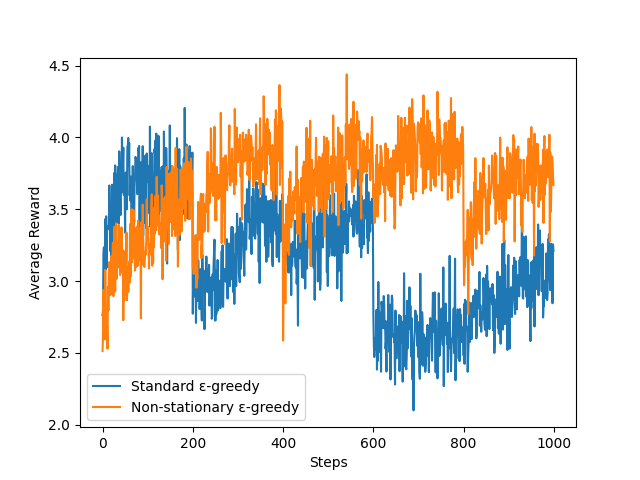
\includegraphics[width=0.8\textwidth]{Figure1MAB.png}
    \caption{Comparison of standard $\epsilon$-greedy and non-stationary $\epsilon$-greedy over 1000 steps.}
    \label{fig:mab_results}
\end{figure}

\end{document}